\section{False Match Removal} 

Fundamental Matrix estimation from two views plays an important role in 3D Computer Vision. It contains all geometric information about the relative transformation between images. The estimation is actually based on solving a homogeneous linear system where each linear equation is formed by a pair of correspondence feature points. A large number of robust estimation approaches have been proposed to alleviate the influence of outliers to the fundamental matrix estimation. Some of them include the M-estimator method which reduces the effect of outliers by by applying weight functions to transform the problem to a weighted least squares problem. However, the approach needs a good initial estimation and only works under low percentages of outliers.This method is very time-consuming.

Random Sample Consensus or RANSAC \cite{RANSAC}\cite{optimalransac} is a very popular algorithm for Fundamental Matrix Estimation. It uses minimal points set to estimate an initial guess and then the confidence of the estimation is established by testing each point correspondence against the model with an inlier set, which is determined by choosing points that have error below a given threshold. After that, a new fundamental matrix is estimated by the inlier set, thus iteratively the RANSAC algorithm attempts to find a solution that maximizes the amount of inlier set.

Re-projection error is adopted in this approach\cite{ming} rather than the widely used algebraic error for confidence evaluation purposes.  An assumption is made of gaussian noise present in each image and the reprojection error of point correspondence can be described by a chi-square distribution. The outliers are eliminated by a 3-sigma principle.

For Robust Fundamental Matrix Estimation, an Eight-point linear algorithm is used, where  estimation from a set of point correspondences between two images is performed. Given a set of two images \textit{I} and \textit{I'}, suppose $x_i \in \textit{I}$ and $x'_{i} \in \textit{I'} $ are a pair of corresponding homogeneous points between the two images, The fundamental matrix \textbf{F} satisfies the following equation:

\begin{center}
	$x^{'T}_i \textbf{F} x_i  = 0$
\end{center}

where the fundamental matrix is a 3 X 3 homogeneous matrix defined up to scale. Each pair of point correspondence yield one linear constraint for the entries of \textbf{F}. Thus the estimation of the fundamental matrix can be done with eight point pairs. When more correspondences are available, the fundamental matrix can be estimated via least squares. 

To evaluate the error for each pair of point correspondence, a perspective 3D reprojection of all the corresponding points can be obtained via triangulations. The reconstructed 3D points can be reprojected back to the two images via the camera matrices. let us suppose $\mathbf{\hat{x}}_i$ and $\mathbf{\hat{x}}'_i$ are the reprojected images of point $i$, the 2D reprojection error of the corresponding point is defined as
\begin{equation}
e_{r}(i) = \frac{1}{2} \sum \|\mathbf{x}_i-\mathbf{\hat{x}}_i\|^2_F + \|\mathbf{x}'_i-\mathbf{\hat{x}}'^2_i\|_F, \;\;\;s.t.\;\;\; 
\mathbf{\hat{x}}'^T_i \mathbf{F} \mathbf{\hat{x}}_i=0 \;\;\; \forall i
\end{equation}


The 2D reprojection error is proven to be more superior to other geometric errors. Optimal triangulation is a linear triangulation method which converts the least-square function to a one parameter function and finds a global optimal solution.

Now, for the strategy for outlier detection, it is being assumed that the image noise is modeled by Gaussian distribution. Through intensive simulations, it is being found that the reprojection errors of outliers are usually greatly larger than those of inliers. As a result, these outliers can be identified using 3-sigma principle. Points with reprojection errors larger than the triple variance of all the reprojection error can be classified as outliers. Based on robust statistics \cite{ming}, we can obtain a robust standard deviation of the reprojection errors by the following equation.

\begin{equation}
\sigma = 1.4826 \Big(1+\frac{5}{n-q}\Big)\text{median}_i|e^r_i|
\end{equation}

The above equation is the median absolute deviation (MAD) scale estimate.
The first number is obtained from the inverse of the cumulative normal distribution,
and the term (1 + 5 ) is the finite sample correction factor with the total number of n−q
parameters q = 8 and n the total number of features. According to the distribution model, we distinguish the inliers from their reprojection errors of each pair of corresponding points. The points whose reprojection errors are less than 3σ are deemed as inliers, since 99.14{\%} of the data points lies within 3$\sigma$ under the assumption of the Gaussian distribution error model.

The  Fast and Robust Algorithm is as follows:

1. Normalize the coordinates of all matching points; 

2. Estimate an initial fundamental matrix using eight-point linear algorithm; 

3. Compute the reprojection error and determine an outlier threshold; 

4. Re-estimate the fundamental matrix using the inliers detected in step 3; 

5. Repeat the steps 3 and 4 one time to refine the inlier set; 

6. Estimate the optimal fundamental matrix using the inliers obtained in step 5. 

\begin{figure}[b]
	\begin{center}
	\DeclareGraphicsExtensions{.pdf,.png,.jpg}
	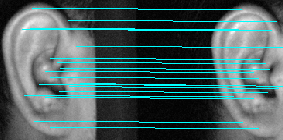
\includegraphics[width=0.7\textwidth]{Figures/Figure22}
	\caption{Feature Point Matches after Outlier Detection}
	\label{fig:Figure22}
	\end{center}
\end{figure}

After simulations are being carried out, it has been seen that the number of matching keypoints decreases after the outlier detection. As shown in Figure \ref{fig:Figure22}, the number of keypoints obtained by SIFT was 27, but after False Matches are removed via the 3-$\sigma$ principle, the number of proper matches come down to 22. Thus making the algorithm more robust to false matches.


